\documentclass[9pt]{beamer}

\usetheme[progressbar=frametitle]{metropolis}
\usepackage[italian]{babel}

\usepackage{paralist}

\usepackage{appendixnumberbeamer}

\usepackage{amsmath}

\usepackage{booktabs}
\usepackage[scale=2]{ccicons}

\usepackage{pgfplots}
\usepgfplotslibrary{dateplot}

\usepackage{xspace}
\newcommand{\themename}{\textbf{\textsc{metropolis}}\xspace}

\title{TSP con pick up and delivery}
\subtitle{Progetto del corso di Ricerca Operativa}
\date{13 dicembre 2022}
\author{Michele Vaccari - Matricola 121955}
\institute{Università degli studi di Ferrara\\Corso di laurea magistrale in Ingegneria Informatica e dell'Automazione\\AA 2020-2021}

% logo of my university
\titlegraphic{%
  \begin{picture}(0,0)
    \put(305,0){\makebox(0,0)[rt]{
\includegraphics[width=4cm]{../images/logo-unife}}}
  \end{picture}}

\begin{document}

\maketitle

\begin{frame}{Indice}
  \setbeamertemplate{section in toc}[sections numbered]
  \tableofcontents
\end{frame}

\section{Introduzione}

\subsection{Descrizione del problema}
\begin{frame}{\subsecname}

	\metroset{block=fill}
	\begin{block}{Progettino 24 - TSP con pick up and delivery (1 persona)}
		A partire dalla base (nodo $0$ del grafo) un corriere deve soddisfare $n$ richieste di prelievo e consegna di documenti:
		\begin{compactitem}
			\item 	ogni documento è prelevato in un nodo e consegnato in un altro nodo;
			\item ogni nodo è riferito a una singola richiesta, ma nel tragitto tra punto di prelievo e consegna si possono prelevare/consegnare altri documenti.
		\end{compactitem}
		Noto il tempo di percorrenza dei singoli archi, si vuole minimizzare la durata del percorso, con partenza e rientro al deposito.
	\end{block}

\end{frame}

\subsection{Un esempio di istanza}
\begin{frame}{\subsecname}

	\begin{figure}[h]
		\centering
		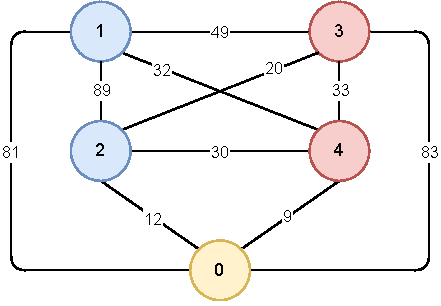
\includegraphics[width=0.6\textwidth]
		{../images/graph-tsppd-with-two-customers}	
		\caption{Istanza con 2 richieste di prelievo e consegna}
	\end{figure}

\end{frame}

\section{Modello matematico per S-TSPPD}
\begin{frame}[allowframebreaks]{Notazione}
	\begin{itemize}
		\item
		Numero di richieste di prelievo e consegna: $n$
		
		\item
		Nodi di pickup: $V_P = \{1, \dots, n\}$
		
		\item
		Nodi di delivery: $V_D = \{n+1, \dots, 2n\}$
		
		\item
		Una richiesta è identificata con la coppia di nodi $(i,n+i)$ e $i$ deve precedere $n+i$ in un percorso ammissibile
		
		\item
		$V$ è definito come l'unione di $V_P$ e $V_D$ con l'aggiunta del nodo di deposito $\{0\}$
		
		\item
		$E_{PD}$ è l'insieme degli archi che connettono $V_P \cup V_D$
	
		\item
		$E$ è l'unione di $E_{PD}$ con tutti gli archi ammissibili che collegano il nodo di deposito
		
		\item
		Il grafo $G=(V,E)$ comprende tutti i nodi e gli archi necessari per descrivere il S-TSPPD (il grafo è completo)
		\[ V=\{0\} \cup V_P \cup V_D \]
		\[ E = \{ (0,i) | i \in V_P \} \cup \{ (0,i) | i \in V_D \} \cup E_{PD} \]
		
		L'insieme degli archi $E$ è definito in modo tale da includere solo archi ammissibili.
		In altre parole, non è possibile che un percorso TSPPD inizi con una consegna o finisca con un prelievo.
		
		\item
		Ogni arco $(i,j) \in E$ è uguale all'arco $(j, i)$

		\item
		Ogni arco ha gli stessi costi e variabili

		\item
		$c_{ij}$ è un costo non negativo per ogni arco $(i,j) \in E$

		\item
		$x_{ij} \in \{ 0, 1 \}$ è una variabile decisionale binaria per ogni $(i, j) \in E$ con il valore $x_{ij} = 1$ se l'arco $(i, j)$ è in una soluzione e $0$ altrimenti

		\item
		$\delta(S) = \{ (i, j) \in E | i \in S, j \notin S$ è il taglio contenente gli archi che collegano $S \subset V$ e $S^* \subset V$ 

		\item
		Per qualsiasi nodo $i \in V, \delta(i) = \delta( \{ i \})$
	\end{itemize}
\end{frame}

\begin{frame}{Modello matematico}

     	\[ min{ \sum_{(i,j) \in E} c_i x_{ij}} \]
	tale che
	\begin{enumerate}
		\item
		\label{stsppd-c1}
		$x_0 = 1$

		\item
		\label{stsppd-c2}
		$x(\delta(i)) = 2 \quad \forall i \in V$

		\item
		\label{stsppd-c3}
		$x(\delta(i)) \geq 2 \quad \forall S \subset V$
	
		\item
		\label{stsppd-c4}
		$x(\delta(i)) \geq 4 \quad \forall S \subset V, \{0, n+i\} \subset S, \{0,i\} \subset V \setminus S$

		\item
		$x_{ij} \in \{0,1\} \quad (i,j) \in E$
	\end{enumerate}
	
	\footnotesize
	Il vincolo \ref{stsppd-c1} richiede che l'arco che collega il nodo di deposito faccia parte di qualsiasi soluzione ammissibile. \\
	Il vincolo \ref{stsppd-c2} richiede che ogni nodo entri ed esca in tutti i percorsi ammissibili, ma di per sé lascia aperta la possibilità di sotto-tour, formando una rappresentazione completa del TSP. \\
	Il vincolo \ref{stsppd-c3} consente di eliminare i sotto-tour, formando una rappresentazione completa del TSP. \\
	Il vincolo \ref{stsppd-c4} richiede che i ritiri avvengano prima delle rispettive consegne

\end{frame}

\section{Modello matematico per A-TSPPD}
\begin{frame}[allowframebreaks]{Notazione}
	\begin{itemize}
		\item
		Numero di richieste di prelievo e consegna: $n$
		
		\item
		Nodi di pickup: $N_P = \{1, \dots, n\}$
		
		\item
		Nodi di delivery: $N_D = \{n+1, \dots, 2n\}$
		
		\item
		Una richiesta è identificata con la coppia di nodi $(i,n+i)$ e $i$ deve precedere $n+i$ in un percorso ammissibile
		
		\item
		$N$ è definito come l'unione di $N_P$ e $N_D$ con l'aggiunta del nodo di deposito $\{0\}$
		
		\item
		$A_{PD}$ è l'insieme degli archi \emph{orientati} che connettono $N_P \cup N_D$
	
		\item
		$A$ è l'unione di $A_{PD}$ con tutti gli archi \emph{orientati} ammissibili che collegano il nodo di deposito
		
		\item
		Il grafo $G=(N,A)$ comprende tutti i nodi e gli archi necessari per descrivere il A-TSPPD (il grafo è completo)
		\begin{equation*}
			\begin{aligned}
			N= & \{0\} \cup N_P \cup N_D \\
			A = & \{ (0,i) | i \in N_P \} \\
			& \cup \{ (i,0) | i \in N_D \} \\
			& \cup \{ (i,j) | i \in N_P , j \in ( N_P \cup N_D ) \setminus \{ i \} \} \\
			& \cup \{ ( n + i, j) | i \in N_P , j \in (N_P \cup N_D ) \setminus \{ i , n + i \} \}
			\end{aligned}
		\end{equation*}
		
		L'insieme degli archi $A$ è definito in modo tale da includere solo archi ammissibili.
		In altre parole, non è possibile che un percorso TSPPD inizi con una consegna o finisca con un prelievo.

		\item
		$c_{ij}$ è un costo non negativo per ogni arco $(i,j) \in A$

		\item
		$x_{ij} \in \{ 0, 1 \}$ è una variabile decisionale binaria per ogni $(i, j) \in A$ con il valore $x_{ij} = 1$ se l'arco $(i, j)$ è in una soluzione e $0$ altrimenti

		\item
		$\delta(S) = \{ (i, j) \in A | i \in S, j \notin S$ è il taglio contenente gli archi che collegano $S \subset N$ e $S^* \subset N$ 

		\item
		Per qualsiasi nodo $i \in N, \delta(i) = \delta( \{ i \})$
	\end{itemize}
\end{frame}

\begin{frame}{Modello matematico}

     	\[ min{ \sum_{(i,j) \in A} c_i x_{ij}} \]
	tale che
	\begin{enumerate}
		\item
		\label{atsppd-c1}
		$\sum_{(i,j) \in A} x_{ij} = 1 \quad \forall i \in N$

		\item
		\label{atsppd-c2}
		$\sum_{(i,j) \in A} x_{ij} = 1 \quad \forall j \in N$

		\item
		\label{atsppd-c3}
		$x(\delta(S)) \geq 1 \quad \forall S \subset N$
	
		\item
		\label{atsppd-c4}
		$x(\delta(i)) \geq 4 \quad \forall S \subset N, \{0, n+i\} \subset S, \{0,i\} \subset N \setminus S$

		\item
		$x_{ij} \in \{0,1\} \quad (i,j) \in A$
	\end{enumerate}
	
	\footnotesize
	I vincoli \ref{atsppd-c1} e \ref{atsppd-c2} richiedono che ogni nodo preceda e segua direttamente un altro nodo. \\
	Il vincolo \ref{atsppd-c3} consente di eliminare i sotto-tour, formando una rappresentazione completa del TSP. \\
	Il vincolo \ref{atsppd-c4} richiede che i ritiri avvengano prima delle rispettive consegne (è uguale al vincolo \ref{stsppd-c4} del S-TSPPD)

\end{frame}

%\begin{frame}[allowframebreaks]{Considerazioni sul problerma}
%	Questo problema di ottimizzazione è NP-hard, poiché coincide con il TSP quando la capacità del veicolo è sufficientemente grande.
%	Anche il problema di verificare se esiste una soluzione ammissibile è un problema fortemente NP-hard, dato che il problema della 3-partizione è un caso particolare (si veda [10] per i dettagli).
%\end{frame}

%\begin{frame}[allowframebreaks]{Interpretazione dei risultati del modello teorico nel problema reale}
%\end{frame}

\begin{frame}[standout]
Grazie per l'attenzione
\end{frame}

\end{document}